%definira klasu dokumenta 
\documentclass[12pt]{report} 

%prostor izmedu naredbi \documentclass i \begin{document} se zove uvod. U njemu se nalaze naredbe koje se odnose na cijeli dokument

%osnovni LaTex ne može riješiti sve probleme, pa se koriste različiti paketi koji olakšavaju izradu željenog dokumenta
\usepackage[croatian]{babel} 
\usepackage{amssymb}
\usepackage{amsmath}
\usepackage{txfonts}
\usepackage{mathdots}
\usepackage{titlesec}
\usepackage{array}
\usepackage{lastpage}
\usepackage{etoolbox}
\usepackage{tabularray}
\usepackage{color, colortbl}
\usepackage{adjustbox}
\usepackage{geometry}
\usepackage[classicReIm]{kpfonts}
\usepackage{hyperref}
\usepackage{fancyhdr}

\usepackage{float}
\usepackage{setspace}
\restylefloat{table}


\patchcmd{\chapter}{\thispagestyle{plain}}{\thispagestyle{fancy}}{}{} %redefiniranje stila stranice u paketu fancyhdr

%oblik naslova poglavlja
\titleformat{\chapter}{\normalfont\huge\bfseries}{\thechapter.}{20pt}{\Huge}
\titlespacing{\chapter}{0pt}{0pt}{40pt}


\linespread{1.3} %razmak između redaka

\geometry{a4paper, left=1in, top=1in,}  %oblik stranice

\hypersetup{ colorlinks, citecolor=black, filecolor=black, linkcolor=black,	urlcolor=black }   %izgled poveznice


%prored smanjen između redaka u nabrajanjima i popisima
\newenvironment{packed_enum}{
	\begin{enumerate}
		\setlength{\itemsep}{0pt}
		\setlength{\parskip}{0pt}
		\setlength{\parsep}{0pt}
	}{\end{enumerate}}

\newenvironment{packed_item}{
	\begin{itemize}
		\setlength{\itemsep}{0pt}
		\setlength{\parskip}{0pt}
		\setlength{\parsep}{0pt}
	}{\end{itemize}}




%boja za privatni i udaljeni kljuc u tablicama
\definecolor{LightBlue}{rgb}{0.9,0.9,1}
\definecolor{LightGreen}{rgb}{0.9,1,0.9}

%Promjena teksta za dugačke tablice
\DefTblrTemplate{contfoot-text}{normal}{Nastavljeno na idućoj stranici}
\SetTblrTemplate{contfoot-text}{normal}
\DefTblrTemplate{conthead-text}{normal}{(Nastavljeno)}
\SetTblrTemplate{conthead-text}{normal}
\DefTblrTemplate{middlehead,lasthead}{normal}{Nastavljeno od prethodne stranice}
\SetTblrTemplate{middlehead,lasthead}{normal}

%podesavanje zaglavlja i podnožja

\pagestyle{fancy}
\lhead{Programsko inženjerstvo}
\rhead{Darivanje krvi}
\lfoot{WeAreAdults}
\cfoot{stranica \thepage/\pageref{LastPage}}
\rfoot{\today}
\renewcommand{\headrulewidth}{0.2pt}
\renewcommand{\footrulewidth}{0.2pt}


\begin{document} 
	
	
	
	\begin{titlepage}
		\begin{center}
			\vspace*{\stretch{1.0}} %u kombinaciji s ostalim \vspace naredbama definira razmak između redaka teksta
			\LARGE Programsko inženjerstvo\\
			\large Ak. god. 2023./2024.\\
			
			\vspace*{\stretch{3.0}}
			
			\huge Darivanje krvi\\
			\Large Dokumentacija, Rev. \textit{1}\\
			
			\vspace*{\stretch{12.0}}
			\normalsize
			Grupa: \textit{WeAreAdults}\\
			Voditelj: \textit{Iva Rengel}\\
			
			
			\vspace*{\stretch{1.0}}
			Datum predaje: \textit{$<$dan$>$. $<$mjesec$>$. $<$godina$>$.}\\
	
			\vspace*{\stretch{4.0}}
			
			Nastavnik: \textit{Vlado Sruk}\\
		
		\end{center}

	
	\end{titlepage}

	
	\tableofcontents


	\chapter{Dnevnik promjena dokumentacije}
		
		\textbf{\textit{Kontinuirano osvježavanje}}\\
				
		
		\begin{longtblr}[
				label=none
			]{
				width = \textwidth, 
				colspec={|X[2]|X[13]|X[3]|X[3]|}, 
				rowhead = 1
			}
			\hline
			\textbf{Rev.}	& \textbf{Opis promjene/dodatka} & \textbf{Autori} & \textbf{Datum}\\[3pt] \hline
			0.1 & Napravljen predložak.	& * & 22.08.2013. 		\\[3pt] \hline 
			0.2	& Dopisane upute za povijest dokumentacije.\newline Dodane reference. & * & 24.08.2013. 	\\[3pt] \hline 
			0.5 & Dodan \textit{Use Case} dijagram i jedan sekvencijski dijagram, funkcionalni i nefunkcionalni zahtjevi i dodatak A & * & 25.08.2013. \\[3pt] \hline 
			0.6 & Arhitektura i dizajn sustava, algoritmi i strukture podataka & * & 26.08.2013. \\[3pt] \hline 
			0.8 & Povijest rada i trenutni status implementacije,\newline Zaključci i plan daljnjeg rada & * & 28.08.2013. \\[3pt] \hline 
			0.9 & Opisi obrazaca uporabe & * & 07.09.2013. \\[3pt] \hline 
			0.10 & Preveden uvod & * & 08.09.2013. \\[3pt] \hline 
			0.11 & Sekvencijski dijagrami & * & 09.09.2013. \\[3pt] \hline 
			0.12.1 & Započeo dijagrame razreda & * & 10.09.2013. \\[3pt] \hline 
			0.12.2 & Nastavak dijagrama razreda & * & 11.09.2013. \\[3pt] \hline 
			\textbf{1.0} & Verzija samo s bitnim dijelovima za 1. ciklus & * & 11.09.2013. \\[3pt] \hline 
			1.1 & Uređivanje teksta -- funkcionalni i nefunkcionalni zahtjevi & * \newline * & 14.09.2013. \\[3pt] \hline 
			1.2 & Manje izmjene:Timer - Brojilo vremena & * & 15.09.2013. \\[3pt] \hline 
			1.3 & Popravljeni dijagrami obrazaca uporabe & * & 15.09.2013. \\[3pt] \hline 
			1.5 & Generalna revizija strukture dokumenta & * & 19.09.2013. \\[3pt] \hline 
			1.5.1 & Manja revizija (dijagram razmještaja) & * & 20.09.2013. \\[3pt] \hline 
			\textbf{2.0} & Konačni tekst predloška dokumentacije  & * & 28.09.2013. \\[3pt] \hline 
			&  &  & \\[3pt] \hline	
		\end{longtblr}
	
	
		\textit{Moraju postojati glavne revizije dokumenata 1.0 i 2.0 na kraju prvog i drugog ciklusa. Između tih revizija mogu postojati manje revizije već prema tome kako se dokument bude nadopunjavao. Očekuje se da nakon svake značajnije promjene (dodatka, izmjene, uklanjanja dijelova teksta i popratnih grafičkih sadržaja) dokumenta se to zabilježi kao revizija. Npr., revizije unutar prvog ciklusa će imati oznake 0.1, 0.2, …, 0.9, 0.10, 0.11.. sve do konačne revizije prvog ciklusa 1.0. U drugom ciklusu se nastavlja s revizijama 1.1, 1.2, itd.}
	\chapter{Opis projektnog zadatka}
		
		\textbf{\textit{dio 1. revizije}}\\
		
		\textit{Na osnovi projektnog zadatka detaljno opisati korisničke zahtjeve. Što jasnije opisati cilj projektnog zadatka, razraditi problematiku zadatka, dodati nove aspekte problema i potencijalnih rješenja. Očekuje se minimalno 3, a poželjno 4-5 stranica opisa.	Teme koje treba dodatno razraditi u ovom poglavlju su:}
		\begin{packed_item}
			\item \textit{potencijalna korist ovog projekta}
			\item \textit{postojeća slična rješenja (istražiti i ukratko opisati razlike u odnosu na zadani zadatak). Dodajte slike koja predočavaju slična rješenja.}
			\item \textit{skup korisnika koji bi mogao biti zainteresiran za ostvareno rješenje.}
			\item \textit{mogućnost prilagodbe rješenja }
			\item \textit{opseg projektnog zadatka}
			\item \textit{moguće nadogradnje projektnog zadatka}
		\end{packed_item}
		
		\textit{Za pomoć pogledati reference navedene u poglavlju „Popis literature“, a po potrebi konzultirati sadržaj na internetu koji nudi dobre smjernice u tom pogledu.}
		\eject
		
		\section{Primjeri u \LaTeX u}
		
		\textit{Ovo potpoglavlje izbrisati.}\\

		U nastavku se nalaze različiti primjeri kako koristiti osnovne funkcionalnosti \LaTeX a koje su potrebne za izradu dokumentacije. Za dodatnu pomoć obratiti se asistentu na projektu ili potražiti upute na sljedećim web sjedištima:
		\begin{itemize}
			\item Upute za izradu diplomskog rada u \LaTeX u - \url{https://www.fer.unizg.hr/_download/repository/LaTeX-upute.pdf}
			\item \LaTeX\ projekt - \url{https://www.latex-project.org/help/}
			\item StackExchange za Tex - \url{https://tex.stackexchange.com/}\\
		
		\end{itemize} 	


		
		\noindent \underbar{podcrtani tekst}, \textbf{podebljani tekst}, 	\textit{nagnuti tekst}\\
		\noindent \normalsize primjer \large primjer \Large primjer \LARGE {primjer} \huge {primjer} \Huge primjer \normalsize
				
		\begin{packed_item}
			
			\item  primjer
			\item  primjer
			\item  primjer
			\item[] \begin{packed_enum}
				\item primjer
				\item[] \begin{packed_enum}
					\item[1.a] primjer
					\item[b] primjer
				\end{packed_enum}
				\item primjer
			\end{packed_enum}
			
		\end{packed_item}
		
		\noindent primjer url-a: \url{https://www.fer.unizg.hr/predmet/proinz/projekt}
		
		\noindent posebni znakovi: \# \$ \% \& \{ \} \_ 
		$|$ $<$ $>$ 
		\^{} 
		\~{} 
		$\backslash$ 
		
		
		\begin{longtblr}[
			label=none,
			entry=none
			]{
				width = \textwidth,
				colspec={|X[8,l]|X[8, l]|X[16, l]|}, 
				rowhead = 1,
			} %definicija širine tablice, širine stupaca, poravnanje i broja redaka naslova tablice
			\hline \SetCell[c=3]{c}{\textbf{naslov unutar tablice}}	 \\ \hline[3pt]
			\SetCell{LightGreen}IDKorisnik & INT	&  	Lorem ipsum dolor sit amet, consectetur adipiscing elit, sed do eiusmod  	\\ \hline
			korisnickoIme	& VARCHAR &   	\\ \hline 
			email & VARCHAR &   \\ \hline 
			ime & VARCHAR	&  		\\ \hline 
			\SetCell{LightBlue} primjer	& VARCHAR &   	\\ \hline 
		\end{longtblr}
		

		\begin{longtblr}[
				caption = {Naslov s referencom izvan tablice},
				entry = {Short Caption},
			]{
				width = \textwidth, 
				colspec = {|X[8,l]|X[8,l]|X[16,l]|}, 
				rowhead = 1,
			}
			\hline
			\SetCell{LightGreen}IDKorisnik & INT	&  	Lorem ipsum dolor sit amet, consectetur adipiscing elit, sed do eiusmod  	\\ \hline
			korisnickoIme	& VARCHAR &   	\\ \hline 
			email & VARCHAR &   \\ \hline 
			ime & VARCHAR	&  		\\ \hline 
			\SetCell{LightBlue} primjer	& VARCHAR &   	\\ \hline 
		\end{longtblr}
	


		
		
		%unos slike
		\begin{figure}[H]
			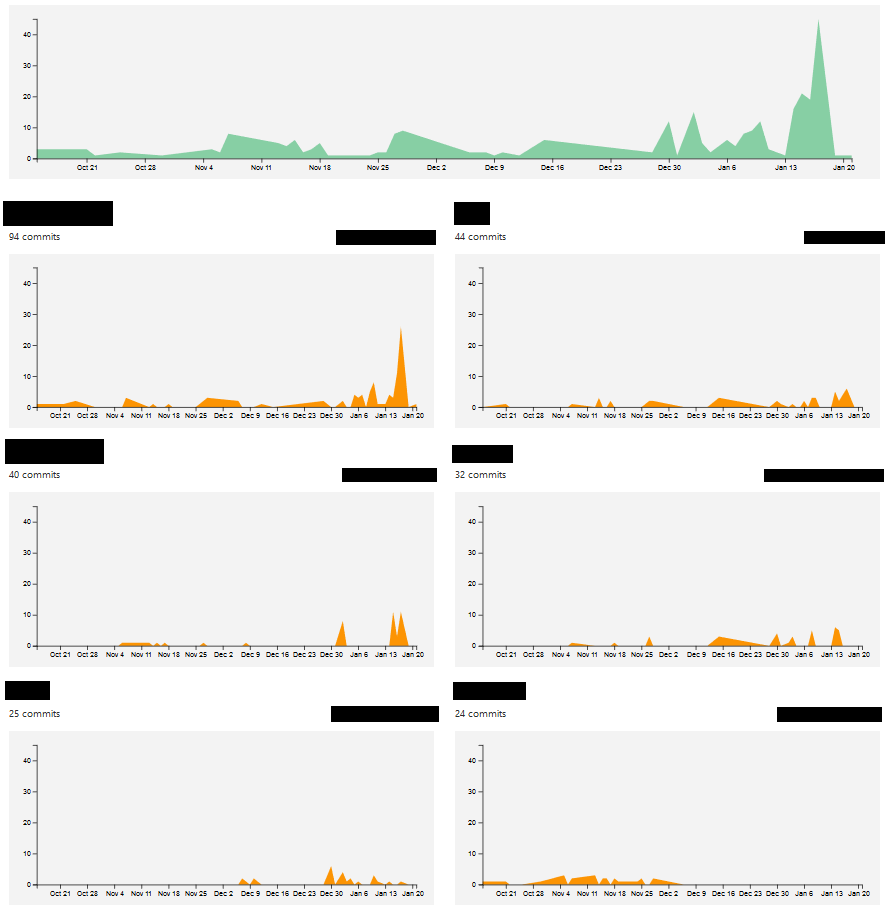
\includegraphics[scale=0.4]{slike/aktivnost.PNG} %veličina slike u odnosu na originalnu datoteku i pozicija slike
			\centering
			\caption{Primjer slike s potpisom}
			\label{fig:promjene}
		\end{figure}
		
		\begin{figure}[H]
			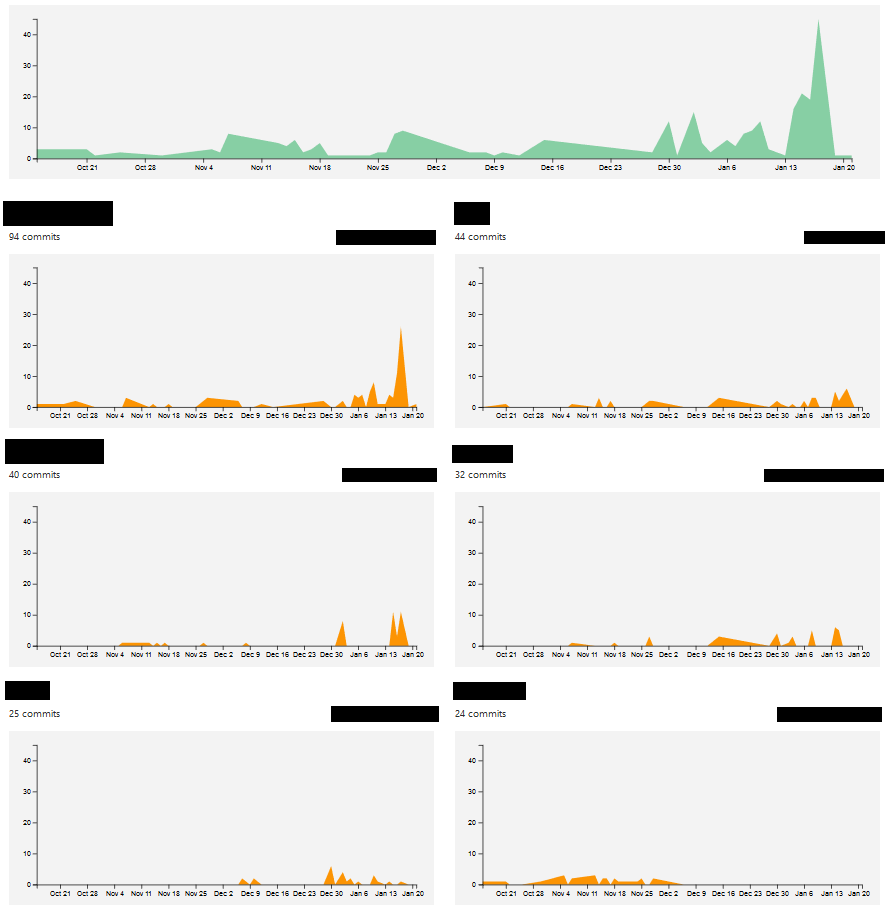
\includegraphics[width=\textwidth]{slike/aktivnost.PNG} %veličina u odnosu na širinu linije
			\caption{Primjer slike s potpisom 2}
			\label{fig:promjene2} %label mora biti drugaciji za svaku sliku
		\end{figure}
		
		Referenciranje slike \ref{fig:promjene2} u tekstu.
		
		\eject
		
	
	\chapter{Specifikacija programske potpore}
		
	\section{Funkcionalni zahtjevi}
			
			\textbf{\textit{dio 1. revizije}}\\
			
			\textit{Navesti \textbf{dionike} koji imaju \textbf{interes u ovom sustavu} ili  \textbf{su nositelji odgovornosti}. To su prije svega korisnici, ali i administratori sustava, naručitelji, razvojni tim.}\\
				
			\textit{Navesti \textbf{aktore} koji izravno \textbf{koriste} ili \textbf{komuniciraju sa sustavom}. Oni mogu imati inicijatorsku ulogu, tj. započinju određene procese u sustavu ili samo sudioničku ulogu, tj. obavljaju određeni posao. Za svakog aktora navesti funkcionalne zahtjeve koji se na njega odnose.}\\
			
			
			\noindent \textbf{Dionici:}
			
			\begin{packed_enum}
				
				\item Neregistrirani korisnik (gost)
				\item Registrirani korisnik
				\begin{packed_enum}
					\item Donor Krvi
					\item Zaposlenik Hrvatskog Crvenog Križa (admin)
				\end{packed_enum}
				\item Razvojni tim
				
			\end{packed_enum}
			
			\noindent \textbf{Aktori i njihovi funkcionalni zahtjevi:}
			
			
			\begin{packed_enum}
				\item  \underbar{Korisnik može:}
				
				\begin{packed_enum}
					
					\item Pregledavati stranicu s općim informacijama
					\item Pregledavati stranicu s lokacijama na kojima može darivati krv
					\item Prijaviti u sustav
					\item Registrirati u sustav
					
				\end{packed_enum}
			
				\item  \underbar{Registrirani korisnik može:}
				
				\begin{packed_enum}
					
					\item Pregledati vlastiti profil
					\begin{packed_enum}
						\item Pregledati i uređivati osobne informacije
						\item Pregledati prijavljene rezervacije termina i otkazati ih
						\item Pregledati povijest darivanja krvi
						\item Pregledati dobivene potvrde
					\end{packed_enum}
					\item Registrirati termin za akciju po izboru
					\item Odjaviti se
					
				\end{packed_enum}

				\item  \underbar{Zaposlenik Crvenog Križa (admin) može:}

				\begin{packed_enum}

					\item Dodati nove akcije
					\item Urediti postojeće akcije
					\begin{packed_enum}
						\item Urediti podatke o akciji
						\item Prijevremeno arhivirati akciju
					\end{packed_enum}
					\item Verificirati korisnika
					\item Bilježiti istance davanja krvi

				\end{packed_enum}

			\end{packed_enum}
			
			\eject 
			
			
				
			\subsection{Obrasci uporabe}
				
				\textbf{\textit{dio 1. revizije}}
				
				\subsubsection{Opis obrazaca uporabe}
					\textit{Funkcionalne zahtjeve razraditi u obliku obrazaca uporabe. Svaki obrazac je potrebno razraditi prema donjem predlošku. Ukoliko u nekom koraku može doći do odstupanja, potrebno je to odstupanje opisati i po mogućnosti ponuditi rješenje kojim bi se tijek obrasca vratio na osnovni tijek.}\\
					

					\noindent \underbar{\textbf{UC1-Prijava korisnika}}
					\begin{packed_item}
	
						\item \textbf{Glavni sudionik: }Registrirani korisnik
						\item  \textbf{Cilj:} Prijaviti se u korisnički račun radi pristupa stranici
						\item  \textbf{Sudionici:} Baza podataka
						\item  \textbf{Preduvjet:} Korisnik je registriran
						\item  \textbf{Opis osnovnog tijeka:}
						
						\item[] \begin{packed_enum}
	
							\item Korisnik odabire opciju prijava
							\item Unosi tražene podatke (korisničko ime i lozinku)
							\item Pristup korisničkim funkcijama
						\end{packed_enum}
						
						\item  \textbf{Opis mogućih odstupanja:}
						
						\item[] \begin{packed_item}
	
							\item[2.a] Pogrešno korisničko ime ili lozinka
							\item[] \begin{packed_enum}
								
								\item Sustav obavještava korisnika o pogrešci i vraća ga na stranicu za prijavu kao neregistriranog korisnika
							
							\end{packed_enum}
							
						\end{packed_item}
					\end{packed_item}
				
				
				\noindent \underbar{\textbf{UC2-Pregled akcija darivanja krvi}}
				\begin{packed_item}
					
					\item \textbf{Glavni sudionik: }Neregistrirani korisnik
					\item  \textbf{Cilj:} Pregledati sve dostupne lokacije i termine darivanja krvi
					\item  \textbf{Sudionici:} Baza podataka
					\item  \textbf{Opis osnovnog tijeka:}
					
					\item[] \begin{packed_enum}
						
						\item Korisniku se na karti prikazuju lokacije na kojima je moguće darivati krv (bolnice i akcije Crvenog Križa)
						\item Odabir jedne od prikazanih lokacija
						\item Prikaz adrese i vremena za moguću rezervaciju
						
					\end{packed_enum}
					
				\end{packed_item}
				
				
				
				\noindent \underbar{\textbf{UC3-Pregled informacija}}
				\begin{packed_item}
					
					\item \textbf{Glavni sudionik: }Neregistrirani korisnik
					\item  \textbf{Cilj:} Pregled općih informacija o Crvenom Križu i akcijama darivanja krvi
					\item  \textbf{Sudionici:} -
					\item  \textbf{Opis osnovnog tijeka:}
					
					\item[] \begin{packed_enum}
						
						\item Odabir "O nama" u navigacijskoj traci
						\item Prikaz informacija o Crvenom Križu, njegovoj djelatnosti i akcijama 	 	
						darivanja krvi koje organiziraju
					\end{packed_enum}
					
						
				\end{packed_item}
				
				
				
				\noindent \underbar{\textbf{UC7-Odjava korisnika}}
				\begin{packed_item}
					
					\item \textbf{Glavni sudionik: }Registrirani korisnik
					\item  \textbf{Cilj:} Odjava iz aplikacije nakon završetka rada
					\item  \textbf{Preduvjet:} Korisnik je prijavljen u sustav
					\item  \textbf{Opis osnovnog tijeka:}
					
					\item[] \begin{packed_enum}
						
						\item Odabir opcije "Odjavi se"
						\item Povratak na početni zaslon kao Gost
					
					\end{packed_enum}
					
				\end{packed_item}
				
				
				
				\noindent \underbar{\textbf{UC8-Otkazivanje termina}}
				\begin{packed_item}
					
					\item \textbf{Glavni sudionik: }Registrirani korisnik
					\item  \textbf{Cilj:} Otkazivanje rezerviranog termina
					\item  \textbf{Sudionici:} Baza podataka
					\item  \textbf{Preduvjet:} Korisnik je prijavljen u sustav i ima rezerviran termin
					\item  \textbf{Opis osnovnog tijeka:}
					
					\item[] \begin{packed_enum}
						
						\item Korisnik otvara profilnu stranicu
						\item Pregledava svoje nadolazeće rezervacije
						\item Odabire termin koji želi otkazati i opciju "Otkaži termin"
						\item Od korisnika se traži potvrda
						\item Korisnik potvrđuje akciju
						\item Termin se briše iz Baze podataka i uklanja s Korisnikovog popisa rezervacija
					\end{packed_enum}
					
					\item  \textbf{Opis mogućih odstupanja:}
					
					\item[] \begin{packed_item}
						
						\item[5.a] Korisnik odustaje od akcije
						\item[] \begin{packed_enum}
							
							\item Rezervacija se ne briše i korisnik se vraća na profilnu stranicu
							
						\end{packed_enum}		
						
					\end{packed_item}
				\end{packed_item}
				
				\noindent \underbar{\textbf{UC9-Uređivanje osobnih podataka}}
				\begin{packed_item}
					
					\item \textbf{Glavni sudionik: }Registrirani korisnik
					\item  \textbf{Cilj:} Promjena netočnih osobnih podataka
					\item  \textbf{Sudionici:} Baza podataka
					\item  \textbf{Preduvjet:} Korisnik je prijavljen u sustav
					\item  \textbf{Opis osnovnog tijeka:}
					
					\item[] \begin{packed_enum}
						
						\item Korisnik otvara profilnu stranicu
						\item Odabir opcije "Uređivanje podataka"
						\item Promjena podataka u otvorenom prozoru za uređivanje
						\item Spremanje promjena i ažuriranje Baze podataka
					\end{packed_enum}
					
					\item  \textbf{Opis mogućih odstupanja:}
					
					\item[] \begin{packed_item}
						
						\item[4.a] Korisnik odustaje od promjena
						\item[] \begin{packed_enum}
							
							\item Promjene se ne spremaju i korisnik se vraća na profilnu stranicu
							
						\end{packed_enum}	
						\item[4.b] Korisnik ne sprema promjene
						\item[] \begin{packed_enum}
							
							\item Sustav obavještava korisnika da promjene nisu spremljene
							\item Korisnik sprema promjene i vraća se na profilnu stranicu
						\end{packed_enum}	
						
					\end{packed_item}
				\end{packed_item}
				
				
				\noindent \underbar{\textbf{UC10-Dodavanje akcija}}
				\begin{packed_item}
					
					\item \textbf{Glavni sudionik: }Administrator
					\item  \textbf{Cilj:} Dodavanje akcije Crvenog Križa za darivanje krvi
					\item  \textbf{Sudionici:} Baza podataka
					\item  \textbf{Preduvjet:} Administrator je prijavljen u sustav
					\item  \textbf{Opis osnovnog tijeka:}
					
					\item[] \begin{packed_enum}
						
						\item Administrator odredi lokacije i vrijeme održavanja akcije
						\item Potvrđuje svoje odabir
						
					\end{packed_enum}
					
					\item  \textbf{Opis mogućih odstupanja:}
					
					\item[] \begin{packed_item}
						
						\item[2.a] Administrator nije potvrdio odabir
						\item[] \begin{packed_enum}
							
							\item Sustav upozorava da promjene nisu spremljene
							
						\end{packed_enum}		
						
					\end{packed_item}
				\end{packed_item}
					
					
					
					\noindent \underbar{\textbf{UC11-Uređivanje akcija}}
					\begin{packed_item}
						
						\item \textbf{Glavni sudionik: }Administrator
						\item  \textbf{Cilj:} Uređivanje podataka aktivne akcije
						\item  \textbf{Sudionici:} Baza podataka
						\item  \textbf{Preduvjet:} Administrator je prijavljen, akcija je aktivna
						\item  \textbf{Opis osnovnog tijeka:}
						
						\item[] \begin{packed_enum}
							
							\item Administrator odabire akciju koju želi urediti
							\item Uređuje željene podatke
							\item Potvrđuje promjene
						\end{packed_enum}
						
						\item  \textbf{Opis mogućih odstupanja:}
						
						\item[] \begin{packed_item}
							
							\item[3.a] Administrator nije potvrdio promjene
							\item[] \begin{packed_enum}
								
								\item Sustav upozorava da promjene nisu spremljene
								
							\end{packed_enum}		
							
						\end{packed_item}
					\end{packed_item}
					
					
					\noindent \underbar{\textbf{UC12-Arhiviranje akcija}}
					\begin{packed_item}
						
						\item \textbf{Glavni sudionik: }Administrator
						\item  \textbf{Cilj:} Arhivirati aktivnu akciju
						\item  \textbf{Sudionici:} Baza podataka
						\item  \textbf{Preduvjet:} Administrator je prijavljen, akcija je aktivna
						\item  \textbf{Opis osnovnog tijeka:}
						
						\item[] \begin{packed_enum}
							
							\item Administrator odabire akciju koju želi arhivirati
							\item Potvrđuje odabir
						\end{packed_enum}
						
						\item  \textbf{Opis mogućih odstupanja:}
						
						\item[] \begin{packed_item}
							
							\item[2.a] Administrator nije potvrdio odabir
							\item[] \begin{packed_enum}
								
								\item Sustav upozorava da promjene nisu spremljene
								
							\end{packed_enum}		
							
						\end{packed_item}
					\end{packed_item}
					
					
					\noindent \underbar{\textbf{UC13-Verifikacija kritičnih podataka}}
					\begin{packed_item}
						
						\item \textbf{Glavni sudionik: }Korisnik, Administrator
						\item  \textbf{Cilj:} Verificirati podatke novog korisnika pri registraciji
						\item  \textbf{Sudionici:} Baza podataka
						\item  \textbf{Preduvjet:} Korisnik se registrirao, administrator je prijavljen u sustav
						\item  \textbf{Opis osnovnog tijeka:}
						
						\item[] \begin{packed_enum}
							
							\item Administrator pristupa popisu registriranih korisnika
							\item Za neverificirane korisnike sustav provjerava ima li osoba barem 18 godina, postoji li njezin MBO u Bazi i, ako postoji, odgovara li ime i prezime toj osobi
							\item Pri uspješnoj provjeri omogućava se gumb "Verificiraj"
							\item Administrator klikom na gumb verificira korisnika
						\end{packed_enum}
						
						\item  \textbf{Opis mogućih odstupanja:}
						
						\item[] \begin{packed_item}
							
							\item[4.a] Korisnik ne zadovoljava kriterije
							\item[] \begin{packed_enum}
								
								\item Administrator klikne na gumb "Odbij"
								\item Korisnik se briše s liste neverificiranih korisnika i iz baze podataka
								
							\end{packed_enum}		
							
						\end{packed_item}
					\end{packed_item}
					
					
					\noindent \underbar{\textbf{UC14-Evidentiranje darivanja krvi}}
					\begin{packed_item}
						
						\item \textbf{Glavni sudionik: }Registrirani korisnik, Administrator
						\item  \textbf{Cilj:} Dodati darivanje krvi u povijest darivanja i u bazu podataka
						\item  \textbf{Sudionici:} Baza podataka
						\item  \textbf{Preduvjet:} Korisnik je darovao krv, Administrator je prijavljen
						\item  \textbf{Opis osnovnog tijeka:}
						
						\item[] \begin{packed_enum}
							
							\item Administrator pristupa bazi podataka
							\item Odabire unos novog zapisa
							\item Popunjava obrazac koji traži ime, prezime, mbo, datum i krvnu grupu osobe
							\item Obrazac se validira i podaci se unose u Bazu
						\end{packed_enum}
						
						\item  \textbf{Opis mogućih odstupanja:}
						
						\item[] \begin{packed_item}
							
							\item[4.a] Neki od traženih podataka nije upisan, unesen je datum iz budućnosti, nije unesena odgovarajuća krvna grupa ili je MBO u pogrešnom formatu
							\item[] \begin{packed_enum}
								
								\item Sustav javlja grešku
								
						\end{packed_enum}				
							
						\end{packed_item}
					\end{packed_item}
					
					
					
				\subsubsection{Dijagrami obrazaca uporabe}
					
					\textit{Prikazati odnos aktora i obrazaca uporabe odgovarajućim UML dijagramom. Nije nužno nacrtati sve na jednom dijagramu. Modelirati po razinama apstrakcije i skupovima srodnih funkcionalnosti.}
				\eject		
				
			\subsection{Sekvencijski dijagrami}
				
				\textbf{\textit{dio 1. revizije}}\\
				
				\textit{Nacrtati sekvencijske dijagrame koji modeliraju najvažnije dijelove sustava (max. 4 dijagrama). Ukoliko postoji nedoumica oko odabira, razjasniti s asistentom. Uz svaki dijagram napisati detaljni opis dijagrama.}
				\eject
	
		\section{Ostali zahtjevi}
		
			\textbf{\textit{dio 1. revizije}}\\
		 
			 \textit{Nefunkcionalni zahtjevi i zahtjevi domene primjene dopunjuju funkcionalne zahtjeve. Oni opisuju \textbf{kako se sustav treba ponašati} i koja \textbf{ograničenja} treba poštivati (performanse, korisničko iskustvo, pouzdanost, standardi kvalitete, sigurnost...). Primjeri takvih zahtjeva u Vašem projektu mogu biti: podržani jezici korisničkog sučelja, vrijeme odziva, najveći mogući podržani broj korisnika, podržane web/mobilne platforme, razina zaštite (protokoli komunikacije, kriptiranje...)... Svaki takav zahtjev potrebno je navesti u jednoj ili dvije rečenice.}
			 
			 
			 
	

	\chapter{Arhitektura i dizajn sustava}
		
		\textbf{\textit{dio 1. revizije}}\\

		\textit{ Potrebno je opisati stil arhitekture te identificirati: podsustave, preslikavanje na radnu platformu, spremišta podataka, mrežne protokole, globalni upravljački tok i sklopovsko-programske zahtjeve. Po točkama razraditi i popratiti odgovarajućim skicama:}
	\begin{itemize}
		\item 	\textit{izbor arhitekture temeljem principa oblikovanja pokazanih na predavanjima (objasniti zašto ste baš odabrali takvu arhitekturu)}
		\item 	\textit{organizaciju sustava s najviše razine apstrakcije (npr. klijent-poslužitelj, baza podataka, datotečni sustav, grafičko sučelje)}
		\item 	\textit{organizaciju aplikacije (npr. slojevi frontend i backend, MVC arhitektura) }		
	\end{itemize}
	
	
	
	
	
	\begin{packed_item}
	\item \textbf{Proces odabira arhitekture}
	\end{packed_item}
		U našem je zadatku cilj web aplikacije olakšati darivateljima krvi i Crvenom Križu cijeli proces darivanja krvi: od organiziranja akcija do pronalaženja istih i rezerviranja termina. Specifikacijom dionika i definiranjem funkcionalnih zahtjeva zaključili smo kako naša aplikacija mora imati tri razine: razinu baze podataka, razinu web-aplikacije i razinu klijenta. Tako navedenim razinama korespondiraju tri sloja: sloj pristupa podacima, sloj aplikacijske logike i sloj korisničkog sučelja. Razmatrajući potrebna svojstva, poput smanjivanja nepotrebnih međuovisnosti između modula radi jednostavnosti pri budućim promjenama, hijerarhijske organizacije razina koja omogućava pristup viših razina nižima preko programskog sučelja i grupiranje dijelova programa koji pristupaju i mijenjaju iste podatke te procedura koje se izvode slijedno radi lakšeg snalaženja, odabrali smo višeslojnu arhitekturu temeljenu na klijent-poslužitelj odnosu, najsličniju MVC stilu arhitekture.
	
	\begin{packed_item}
	\item \textbf{Višeslojna arhitektura i MVC stil}
	\end{packed_item}
		Odnos klijent-poslužitelj opisuje međusobni odnos programa koji sudjeluju u aplikaciji, to jest njihovo funkcioniranje prije, tijekom i po završetku komunikacije klijenta i poslužitelja. Aplikacija sadrži tri osnovna sloja: 
	
	\begin{itemize}
	\item[] \begin{packed_enum}
		\item \underbar{Klijentsku komponentu} - sloj s korisničkim sučeljem, predstavljena web preglednikom, služi kao sučelje između klijenta i poslužitelja, omogućava klijentu slanje HTTP zahtjeva i primanje HTTP odgovora, prevoditelj koji web stranicu pisanu u kodu prikazuje u klijentu razumljivom obliku
		\item \underbar{Poslužiteljsku komponentu} - sloj aplikacijske logike, predstavlja web poslužitelj, centar za razmjenu informacija i pružanje usluga, služi za pohranu, obradu i dostavu web stranica klijentu, pokreće web aplikaciju i prosljeđuje joj klijentove zahtjeve, po potrebi pristupa bazi podataka i vraća klijentu odgovor vidljiv u web pregledniku
		\item \underbar{Baza podataka} - sloj za pohranu podataka
	
	\end{packed_enum}
	\end{itemize}
	
	\begin{figure}[H]
		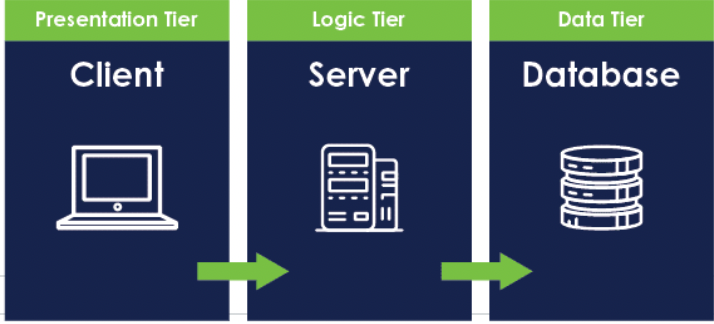
\includegraphics[scale=0.4]{slike/troslojnaArhitektura.png} %veličina slike u odnosu na originalnu datoteku i pozicija slike
		\centering
		\caption{Troslojna arhitektura}
		\label{fig:troslojnaArhitektura}
	\end{figure}
	
	
		Prednost klijent-server arhitekture je mogućnost odvojenog oblikovanja slojeva, što također omogućava “separation of concerns”, to jest svaki sloj brine samo za svoju zadaću i ne brine o funkcionalnostima drugih slojeva, a njihova se međuovisnost ostvaruje komunikacijom pomoću sučelja. 
		Ovako razrađenoj arhitekturi, najsličniji je Model-View-Controller stil. Osnovna je karakteristika ovog stila razdvajanje briga nezavisnim razvojem pojedinih dijelova aplikacije, što omogućuje jednostavnije i učinkovitije testiranje i izmjene dijelova sustava radi njihove dorade te skalabilnost i fleksibilnost cijele aplikacije razvijene na ovakvom principu. Korisničko sučelje je odvojeno od ostatka sustava, a povezanost elemenata se ostvaruje kroz tri sloja: sloja “View” na klijentskoj strani, te slojeva “Model” i “Controller” na poslužiteljskoj strani.
	\begin{packed_item}
		

	\item[] \begin{packed_enum}
		\item \textit{Model (model)} - predstavlja podatke i logiku vezanu za njih, služi za oblikovanje podataka i prilagodbu komunikaciji s bazom
		\item \textit{View (pogled)} - komunikacija s korisnikom i prikaz podataka koje je dobio od upravitelja
		\item \textit{Controller (upravitelj)} - povezuje modele i poglede, na temelju primljenih korisničkih zahtjeva i podataka izvršava potrebne funkcije i formira odgovore
		
	\end{packed_enum}
	\end{packed_item}
	
	\begin{figure}[H]
		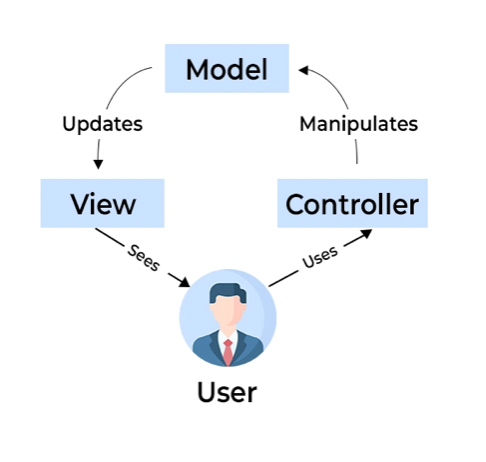
\includegraphics[scale=0.4]{slike/MVC.png} %veličina slike u odnosu na originalnu datoteku i pozicija slike
		\centering
		\caption{MVC stil arhitekture}
		\label{fig:mvc}
	\end{figure}
	
	
		Web aplikacija je podijeljena na front-end i back-end.
		Front-end čini prezentacijski dio aplikacije, to jest ono što korisnik vidi u web pregledniku. Za izradu aplikacije na klijentskoj strani odabrali smo radni okvir React, koji je zasnovan na JavaScriptu i pruža učinkovit razvoj korisničkog sučelja koristeći već gotove web komponente.
		Back-end čini dio sustava u kojem se obrađuju korisnički zahtjevi i vrše potrebne akcije, to jest poslužiteljska strana klijent-server arhitekture. Za njegovu smo izradu odabrali programski jezik Python i radni okvir FastAPI.
		I za razvoj klijentske i za razvoj poslužiteljske strane odabrali smo Visual Studio Code kao radno okruženje.
		
	

				
		\section{Baza podataka}
			
			\textbf{\textit{dio 1. revizije}}\\
			
		\textit{Potrebno je opisati koju vrstu i implementaciju baze podataka ste odabrali, glavne komponente od kojih se sastoji i slično.}
		
			\subsection{Opis tablica}
			

				\textit{Svaku tablicu je potrebno opisati po zadanom predlošku. Lijevo se nalazi točno ime varijable u bazi podataka, u sredini se nalazi tip podataka, a desno se nalazi opis varijable. Svjetlozelenom bojom označite primarni ključ. Svjetlo plavom označite strani ključ}
				
				
				\begin{longtblr}[
					label=none,
					entry=none
					]{
						width = \textwidth,
						colspec={|X[6,l]|X[6, l]|X[20, l]|}, 
						rowhead = 1,
					} %definicija širine tablice, širine stupaca, poravnanje i broja redaka naslova tablice
					\hline \SetCell[c=3]{c}{\textbf{korisnik - ime tablice}}	 \\ \hline[3pt]
					\SetCell{LightGreen}IDKorisnik & INT	&  	Lorem ipsum dolor sit amet, consectetur adipiscing elit, sed do eiusmod  	\\ \hline
					korisnickoIme	& VARCHAR &   	\\ \hline 
					email & VARCHAR &   \\ \hline 
					ime & VARCHAR	&  		\\ \hline 
					\SetCell{LightBlue} primjer	& VARCHAR &   	\\ \hline 
				\end{longtblr}
				
				
			
			\subsection{Dijagram baze podataka}
				\textit{ U ovom potpoglavlju potrebno je umetnuti dijagram baze podataka. Primarni i strani ključevi moraju biti označeni, a tablice povezane. Bazu podataka je potrebno normalizirati. Podsjetite se kolegija "Baze podataka".}
			
			\eject
			
			
		\section{Dijagram razreda}
		
			\textit{Potrebno je priložiti dijagram razreda s pripadajućim opisom. Zbog preglednosti je moguće dijagram razlomiti na više njih, ali moraju biti grupirani prema sličnim razinama apstrakcije i srodnim funkcionalnostima.}\\
			
			\textbf{\textit{dio 1. revizije}}\\
			
			\textit{Prilikom prve predaje projekta, potrebno je priložiti potpuno razrađen dijagram razreda vezan uz \textbf{generičku funkcionalnost} sustava. Ostale funkcionalnosti trebaju biti idejno razrađene u dijagramu sa sljedećim komponentama: nazivi razreda, nazivi metoda i vrste pristupa metodama (npr. javni, zaštićeni), nazivi atributa razreda, veze i odnosi između razreda.}\\
			
			\textbf{\textit{dio 2. revizije}}\\			
			
			\textit{Prilikom druge predaje projekta dijagram razreda i opisi moraju odgovarati stvarnom stanju implementacije}
			
			
			
			\eject
		
		\section{Dijagram stanja}
			
			
			\textbf{\textit{dio 2. revizije}}\\
			
			\textit{Potrebno je priložiti dijagram stanja i opisati ga. Dovoljan je jedan dijagram stanja koji prikazuje \textbf{značajan dio funkcionalnosti} sustava. Na primjer, stanja korisničkog sučelja i tijek korištenja neke ključne funkcionalnosti jesu značajan dio sustava, a registracija i prijava nisu. }
			
			
			\eject 
		
		\section{Dijagram aktivnosti}
			
			\textbf{\textit{dio 2. revizije}}\\
			
			 \textit{Potrebno je priložiti dijagram aktivnosti s pripadajućim opisom. Dijagram aktivnosti treba prikazivati značajan dio sustava.}
			
			\eject
		\section{Dijagram komponenti}
		
			\textbf{\textit{dio 2. revizije}}\\
		
			 \textit{Potrebno je priložiti dijagram komponenti s pripadajućim opisom. Dijagram komponenti treba prikazivati strukturu cijele aplikacije.}
	\chapter{Implementacija i korisničko sučelje}
		
		
		\section{Korištene tehnologije i alati}
		
			\textbf{\textit{dio 2. revizije}}
			
			 \textit{Detaljno navesti sve tehnologije i alate koji su primijenjeni pri izradi dokumentacije i aplikacije. Ukratko ih opisati, te navesti njihovo značenje i mjesto primjene. Za svaki navedeni alat i tehnologiju je potrebno \textbf{navesti internet poveznicu} gdje se mogu preuzeti ili više saznati o njima}.
			
			
			\eject 
		
	
		\section{Ispitivanje programskog rješenja}
			
			\textbf{\textit{dio 2. revizije}}\\
			
			 \textit{U ovom poglavlju je potrebno opisati provedbu ispitivanja implementiranih funkcionalnosti na razini komponenti i na razini cijelog sustava s prikazom odabranih ispitnih slučajeva. Studenti trebaju ispitati temeljnu funkcionalnost i rubne uvjete.}
	
			
			\subsection{Ispitivanje komponenti}
			\textit{Potrebno je provesti ispitivanje jedinica (engl. unit testing) nad razredima koji implementiraju temeljne funkcionalnosti. Razraditi \textbf{minimalno 6 ispitnih slučajeva} u kojima će se ispitati redovni slučajevi, rubni uvjeti te izazivanje pogreške (engl. exception throwing). Poželjno je stvoriti i ispitni slučaj koji koristi funkcionalnosti koje nisu implementirane. Potrebno je priložiti izvorni kôd svih ispitnih slučajeva te prikaz rezultata izvođenja ispita u razvojnom okruženju (prolaz/pad ispita). }
			
			
			
			\subsection{Ispitivanje sustava}
			
			 \textit{Potrebno je provesti i opisati ispitivanje sustava koristeći radni okvir Selenium\footnote{\url{https://www.seleniumhq.org/}}. Razraditi \textbf{minimalno 4 ispitna slučaja} u kojima će se ispitati redovni slučajevi, rubni uvjeti te poziv funkcionalnosti koja nije implementirana/izaziva pogrešku kako bi se vidjelo na koji način sustav reagira kada nešto nije u potpunosti ostvareno. Ispitni slučaj se treba sastojati od ulaza (npr. korisničko ime i lozinka), očekivanog izlaza ili rezultata, koraka ispitivanja i dobivenog izlaza ili rezultata.\\ }
			 
			 \textit{Izradu ispitnih slučajeva pomoću radnog okvira Selenium moguće je provesti pomoću jednog od sljedeća dva alata:}
			 \begin{itemize}
			 	\item \textit{dodatak za preglednik \textbf{Selenium IDE} - snimanje korisnikovih akcija radi automatskog ponavljanja ispita	}
			 	\item \textit{\textbf{Selenium WebDriver} - podrška za pisanje ispita u jezicima Java, C\#, PHP koristeći posebno programsko sučelje.}
			 \end{itemize}
		 	\textit{Detalji o korištenju alata Selenium bit će prikazani na posebnom predavanju tijekom semestra.}
			
			\eject 
		
		
		\section{Dijagram razmještaja}
			
			\textbf{\textit{dio 2. revizije}}
			
			 \textit{Potrebno je umetnuti \textbf{specifikacijski} dijagram razmještaja i opisati ga. Moguće je umjesto specifikacijskog dijagrama razmještaja umetnuti dijagram razmještaja instanci, pod uvjetom da taj dijagram bolje opisuje neki važniji dio sustava.}
			
			\eject 
		
		\section{Upute za puštanje u pogon}
		
			\textbf{\textit{dio 2. revizije}}\\
		
			 \textit{U ovom poglavlju potrebno je dati upute za puštanje u pogon (engl. deployment) ostvarene aplikacije. Na primjer, za web aplikacije, opisati postupak kojim se od izvornog kôda dolazi do potpuno postavljene baze podataka i poslužitelja koji odgovara na upite korisnika. Za mobilnu aplikaciju, postupak kojim se aplikacija izgradi, te postavi na neku od trgovina. Za stolnu (engl. desktop) aplikaciju, postupak kojim se aplikacija instalira na računalo. Ukoliko mobilne i stolne aplikacije komuniciraju s poslužiteljem i/ili bazom podataka, opisati i postupak njihovog postavljanja. Pri izradi uputa preporučuje se \textbf{naglasiti korake instalacije uporabom natuknica} te koristiti što je više moguće \textbf{slike ekrana} (engl. screenshots) kako bi upute bile jasne i jednostavne za slijediti.}
			
			
			 \textit{Dovršenu aplikaciju potrebno je pokrenuti na javno dostupnom poslužitelju. Studentima se preporuča korištenje neke od sljedećih besplatnih usluga: \href{https://aws.amazon.com/}{Amazon AWS}, \href{https://azure.microsoft.com/en-us/}{Microsoft Azure} ili \href{https://www.heroku.com/}{Heroku}. Mobilne aplikacije trebaju biti objavljene na F-Droid, Google Play ili Amazon App trgovini.}
			
			
			\eject 
	\chapter{Zaključak i budući rad}
		
		\textbf{\textit{dio 2. revizije}}\\
		
		 \textit{U ovom poglavlju potrebno je napisati osvrt na vrijeme izrade projektnog zadatka, koji su tehnički izazovi prepoznati, jesu li riješeni ili kako bi mogli biti riješeni, koja su znanja stečena pri izradi projekta, koja bi znanja bila posebno potrebna za brže i kvalitetnije ostvarenje projekta i koje bi bile perspektive za nastavak rada u projektnoj grupi.}
		
		 \textit{Potrebno je točno popisati funkcionalnosti koje nisu implementirane u ostvarenoj aplikaciji.}
		
		\eject 
	\chapter*{Popis literature}
		\addcontentsline{toc}{chapter}{Popis literature}
	 	
 		\textbf{\textit{Kontinuirano osvježavanje}}
	
		\textit{Popisati sve reference i literaturu koja je pomogla pri ostvarivanju projekta.}
		
		
		\begin{enumerate}
			
			
			\item  Programsko inženjerstvo, FER ZEMRIS, \url{http://www.fer.hr/predmet/proinz}
			
			\item  I. Sommerville, "Software engineering", 8th ed, Addison Wesley, 2007.
			
			\item  T.C.Lethbridge, R.Langaniere, "Object-Oriented Software Engineering", 2nd ed. McGraw-Hill, 2005.
			
			\item  I. Marsic, Software engineering book``, Department of Electrical and Computer Engineering, Rutgers University, \url{http://www.ece.rutgers.edu/~marsic/books/SE}
			
			\item  The Unified Modeling Language, \url{https://www.uml-diagrams.org/}
			
			\item  Astah Community, \url{http://astah.net/editions/uml-new}
		\end{enumerate}
		
		 
	
	
	\begingroup
	\renewcommand*\listfigurename{Indeks slika i dijagrama}
	%\renewcommand*\listtablename{Indeks tablica}
	%\let\clearpage\relax
	\listoffigures
	%\vspace{10mm}
	%\listoftables
	\endgroup
	\addcontentsline{toc}{chapter}{Indeks slika i dijagrama}


	
	\eject 
		
	\chapter*{Dodatak: Prikaz aktivnosti grupe}
		\addcontentsline{toc}{chapter}{Dodatak: Prikaz aktivnosti grupe}
		
		\section*{Dnevnik sastajanja}
		
		\textbf{\textit{Kontinuirano osvježavanje}}\\
		
		 \textit{U ovom dijelu potrebno je redovito osvježavati dnevnik sastajanja prema predlošku.}
		
		\begin{packed_enum}
			\item  sastanak
			
			\item[] \begin{packed_item}
				\item Datum: u ovom formatu: \today
				\item Prisustvovali: I.Prezime, I.Prezime
				\item Teme sastanka:
				\begin{packed_item}
					\item  opis prve teme
					\item  opis druge teme
				\end{packed_item}
			\end{packed_item}
			
			\item  sastanak
			\item[] \begin{packed_item}
				\item Datum: u ovom formatu: \today
				\item Prisustvovali: I.Prezime, I.Prezime
				\item Teme sastanka:
				\begin{packed_item}
					\item  opis prve teme
					\item  opis druge teme
				\end{packed_item}
			\end{packed_item}
			
			%
			
		\end{packed_enum}
		
		\eject
		\section*{Tablica aktivnosti}
		
			\textbf{\textit{Kontinuirano osvježavanje}}\\
			
			 \textit{Napomena: Doprinose u aktivnostima treba navesti u satima po članovima grupe po aktivnosti.}

			\begin{longtblr}[
					label=none,
				]{
					vlines,hlines,
					width = \textwidth,
					colspec={X[7, l]X[1, c]X[1, c]X[1, c]X[1, c]X[1, c]X[1, c]X[1, c]}, 
					vline{1} = {1}{text=\clap{}},
					hline{1} = {1}{text=\clap{}},
					rowhead = 1,
				} 
			
				\SetCell[c=1]{c}{} & \SetCell[c=1]{c}{\rotatebox{90}{\textbf{Ime Prezime voditelja}}} & \SetCell[c=1]{c}{\rotatebox{90}{\textbf{Ime Prezime }}} &	\SetCell[c=1]{c}{\rotatebox{90}{\textbf{Ime Prezime }}} & \SetCell[c=1]{c}{\rotatebox{90}{\textbf{Ime Prezime }}} &	\SetCell[c=1]{c}{\rotatebox{90}{\textbf{Ime Prezime }}} & \SetCell[c=1]{c}{\rotatebox{90}{\textbf{Ime Prezime }}} &	\SetCell[c=1]{c}{\rotatebox{90}{\textbf{Ime Prezime }}} \\  
				Upravljanje projektom 		&  &  &  &  &  &  & \\ 
				Opis projektnog zadatka 	&  &  &  &  &  &  & \\ 
				
				Funkcionalni zahtjevi       &  &  &  &  &  &  &  \\ 
				Opis pojedinih obrazaca 	&  &  &  &  &  &  &  \\ 
				Dijagram obrazaca 			&  &  &  &  &  &  &  \\ 
				Sekvencijski dijagrami 		&  &  &  &  &  &  &  \\ 
				Opis ostalih zahtjeva 		&  &  &  &  &  &  &  \\ 

				Arhitektura i dizajn sustava	 &  &  &  &  &  &  &  \\ 
				Baza podataka				&  &  &  &  &  &  &   \\ 
				Dijagram razreda 			&  &  &  &  &  &  &   \\ 
				Dijagram stanja				&  &  &  &  &  &  &  \\ 
				Dijagram aktivnosti 		&  &  &  &  &  &  &  \\ 
				Dijagram komponenti			&  &  &  &  &  &  &  \\ 
				Korištene tehnologije i alati 		&  &  &  &  &  &  &  \\ 
				Ispitivanje programskog rješenja 	&  &  &  &  &  &  &  \\ 
				Dijagram razmještaja			&  &  &  &  &  &  &  \\ 
				Upute za puštanje u pogon 		&  &  &  &  &  &  &  \\  
				Dnevnik sastajanja 			&  &  &  &  &  &  &  \\ 
				Zaključak i budući rad 		&  &  &  &  &  &  &  \\  
				Popis literature 			&  &  &  &  &  &  &  \\  
				&  &  &  &  &  &  &  \\ \hline 
				\textit{Dodatne stavke kako ste podijelili izradu aplikacije} 			&  &  &  &  &  &  &  \\ 
				\textit{npr. izrada početne stranice} 				&  &  &  &  &  &  &  \\  
				\textit{izrada baze podataka} 		 			&  &  &  &  &  &  & \\  
				\textit{spajanje s bazom podataka} 							&  &  &  &  &  &  &  \\ 
				\textit{back end} 							&  &  &  &  &  &  &  \\  
				 							&  &  &  &  &  &  &\\ 
			\end{longtblr}
					
					
		\eject
		\section*{Dijagrami pregleda promjena}
		
		\textbf{\textit{dio 2. revizije}}\\
		
		\textit{Prenijeti dijagram pregleda promjena nad datotekama projekta. Potrebno je na kraju projekta generirane grafove s gitlaba prenijeti u ovo poglavlje dokumentacije. Dijagrami za vlastiti projekt se mogu preuzeti s gitlab.com stranice, u izborniku Repository, pritiskom na stavku Contributors.}
		
	


\end{document} %naredbe i tekst nakon ove naredbe ne ulaze u izgrađen dokument 


